% Options for packages loaded elsewhere
\PassOptionsToPackage{unicode}{hyperref}
\PassOptionsToPackage{hyphens}{url}
%
\documentclass[
  man]{apa6}
\usepackage{amsmath,amssymb}
\usepackage{iftex}
\ifPDFTeX
  \usepackage[T1]{fontenc}
  \usepackage[utf8]{inputenc}
  \usepackage{textcomp} % provide euro and other symbols
\else % if luatex or xetex
  \usepackage{unicode-math} % this also loads fontspec
  \defaultfontfeatures{Scale=MatchLowercase}
  \defaultfontfeatures[\rmfamily]{Ligatures=TeX,Scale=1}
\fi
\usepackage{lmodern}
\ifPDFTeX\else
  % xetex/luatex font selection
\fi
% Use upquote if available, for straight quotes in verbatim environments
\IfFileExists{upquote.sty}{\usepackage{upquote}}{}
\IfFileExists{microtype.sty}{% use microtype if available
  \usepackage[]{microtype}
  \UseMicrotypeSet[protrusion]{basicmath} % disable protrusion for tt fonts
}{}
\makeatletter
\@ifundefined{KOMAClassName}{% if non-KOMA class
  \IfFileExists{parskip.sty}{%
    \usepackage{parskip}
  }{% else
    \setlength{\parindent}{0pt}
    \setlength{\parskip}{6pt plus 2pt minus 1pt}}
}{% if KOMA class
  \KOMAoptions{parskip=half}}
\makeatother
\usepackage{xcolor}
\usepackage{color}
\usepackage{fancyvrb}
\newcommand{\VerbBar}{|}
\newcommand{\VERB}{\Verb[commandchars=\\\{\}]}
\DefineVerbatimEnvironment{Highlighting}{Verbatim}{commandchars=\\\{\}}
% Add ',fontsize=\small' for more characters per line
\usepackage{framed}
\definecolor{shadecolor}{RGB}{248,248,248}
\newenvironment{Shaded}{\begin{snugshade}}{\end{snugshade}}
\newcommand{\AlertTok}[1]{\textcolor[rgb]{0.94,0.16,0.16}{#1}}
\newcommand{\AnnotationTok}[1]{\textcolor[rgb]{0.56,0.35,0.01}{\textbf{\textit{#1}}}}
\newcommand{\AttributeTok}[1]{\textcolor[rgb]{0.13,0.29,0.53}{#1}}
\newcommand{\BaseNTok}[1]{\textcolor[rgb]{0.00,0.00,0.81}{#1}}
\newcommand{\BuiltInTok}[1]{#1}
\newcommand{\CharTok}[1]{\textcolor[rgb]{0.31,0.60,0.02}{#1}}
\newcommand{\CommentTok}[1]{\textcolor[rgb]{0.56,0.35,0.01}{\textit{#1}}}
\newcommand{\CommentVarTok}[1]{\textcolor[rgb]{0.56,0.35,0.01}{\textbf{\textit{#1}}}}
\newcommand{\ConstantTok}[1]{\textcolor[rgb]{0.56,0.35,0.01}{#1}}
\newcommand{\ControlFlowTok}[1]{\textcolor[rgb]{0.13,0.29,0.53}{\textbf{#1}}}
\newcommand{\DataTypeTok}[1]{\textcolor[rgb]{0.13,0.29,0.53}{#1}}
\newcommand{\DecValTok}[1]{\textcolor[rgb]{0.00,0.00,0.81}{#1}}
\newcommand{\DocumentationTok}[1]{\textcolor[rgb]{0.56,0.35,0.01}{\textbf{\textit{#1}}}}
\newcommand{\ErrorTok}[1]{\textcolor[rgb]{0.64,0.00,0.00}{\textbf{#1}}}
\newcommand{\ExtensionTok}[1]{#1}
\newcommand{\FloatTok}[1]{\textcolor[rgb]{0.00,0.00,0.81}{#1}}
\newcommand{\FunctionTok}[1]{\textcolor[rgb]{0.13,0.29,0.53}{\textbf{#1}}}
\newcommand{\ImportTok}[1]{#1}
\newcommand{\InformationTok}[1]{\textcolor[rgb]{0.56,0.35,0.01}{\textbf{\textit{#1}}}}
\newcommand{\KeywordTok}[1]{\textcolor[rgb]{0.13,0.29,0.53}{\textbf{#1}}}
\newcommand{\NormalTok}[1]{#1}
\newcommand{\OperatorTok}[1]{\textcolor[rgb]{0.81,0.36,0.00}{\textbf{#1}}}
\newcommand{\OtherTok}[1]{\textcolor[rgb]{0.56,0.35,0.01}{#1}}
\newcommand{\PreprocessorTok}[1]{\textcolor[rgb]{0.56,0.35,0.01}{\textit{#1}}}
\newcommand{\RegionMarkerTok}[1]{#1}
\newcommand{\SpecialCharTok}[1]{\textcolor[rgb]{0.81,0.36,0.00}{\textbf{#1}}}
\newcommand{\SpecialStringTok}[1]{\textcolor[rgb]{0.31,0.60,0.02}{#1}}
\newcommand{\StringTok}[1]{\textcolor[rgb]{0.31,0.60,0.02}{#1}}
\newcommand{\VariableTok}[1]{\textcolor[rgb]{0.00,0.00,0.00}{#1}}
\newcommand{\VerbatimStringTok}[1]{\textcolor[rgb]{0.31,0.60,0.02}{#1}}
\newcommand{\WarningTok}[1]{\textcolor[rgb]{0.56,0.35,0.01}{\textbf{\textit{#1}}}}
\usepackage{graphicx}
\makeatletter
\def\maxwidth{\ifdim\Gin@nat@width>\linewidth\linewidth\else\Gin@nat@width\fi}
\def\maxheight{\ifdim\Gin@nat@height>\textheight\textheight\else\Gin@nat@height\fi}
\makeatother
% Scale images if necessary, so that they will not overflow the page
% margins by default, and it is still possible to overwrite the defaults
% using explicit options in \includegraphics[width, height, ...]{}
\setkeys{Gin}{width=\maxwidth,height=\maxheight,keepaspectratio}
% Set default figure placement to htbp
\makeatletter
\def\fps@figure{htbp}
\makeatother
\setlength{\emergencystretch}{3em} % prevent overfull lines
\providecommand{\tightlist}{%
  \setlength{\itemsep}{0pt}\setlength{\parskip}{0pt}}
\setcounter{secnumdepth}{-\maxdimen} % remove section numbering
% Make \paragraph and \subparagraph free-standing
\makeatletter
\ifx\paragraph\undefined\else
  \let\oldparagraph\paragraph
  \renewcommand{\paragraph}{
    \@ifstar
      \xxxParagraphStar
      \xxxParagraphNoStar
  }
  \newcommand{\xxxParagraphStar}[1]{\oldparagraph*{#1}\mbox{}}
  \newcommand{\xxxParagraphNoStar}[1]{\oldparagraph{#1}\mbox{}}
\fi
\ifx\subparagraph\undefined\else
  \let\oldsubparagraph\subparagraph
  \renewcommand{\subparagraph}{
    \@ifstar
      \xxxSubParagraphStar
      \xxxSubParagraphNoStar
  }
  \newcommand{\xxxSubParagraphStar}[1]{\oldsubparagraph*{#1}\mbox{}}
  \newcommand{\xxxSubParagraphNoStar}[1]{\oldsubparagraph{#1}\mbox{}}
\fi
\makeatother
% definitions for citeproc citations
\NewDocumentCommand\citeproctext{}{}
\NewDocumentCommand\citeproc{mm}{%
  \begingroup\def\citeproctext{#2}\cite{#1}\endgroup}
\makeatletter
 % allow citations to break across lines
 \let\@cite@ofmt\@firstofone
 % avoid brackets around text for \cite:
 \def\@biblabel#1{}
 \def\@cite#1#2{{#1\if@tempswa , #2\fi}}
\makeatother
\newlength{\cslhangindent}
\setlength{\cslhangindent}{1.5em}
\newlength{\csllabelwidth}
\setlength{\csllabelwidth}{3em}
\newenvironment{CSLReferences}[2] % #1 hanging-indent, #2 entry-spacing
 {\begin{list}{}{%
  \setlength{\itemindent}{0pt}
  \setlength{\leftmargin}{0pt}
  \setlength{\parsep}{0pt}
  % turn on hanging indent if param 1 is 1
  \ifodd #1
   \setlength{\leftmargin}{\cslhangindent}
   \setlength{\itemindent}{-1\cslhangindent}
  \fi
  % set entry spacing
  \setlength{\itemsep}{#2\baselineskip}}}
 {\end{list}}
\usepackage{calc}
\newcommand{\CSLBlock}[1]{\hfill\break\parbox[t]{\linewidth}{\strut\ignorespaces#1\strut}}
\newcommand{\CSLLeftMargin}[1]{\parbox[t]{\csllabelwidth}{\strut#1\strut}}
\newcommand{\CSLRightInline}[1]{\parbox[t]{\linewidth - \csllabelwidth}{\strut#1\strut}}
\newcommand{\CSLIndent}[1]{\hspace{\cslhangindent}#1}
\ifLuaTeX
\usepackage[bidi=basic]{babel}
\else
\usepackage[bidi=default]{babel}
\fi
\babelprovide[main,import]{english}
% get rid of language-specific shorthands (see #6817):
\let\LanguageShortHands\languageshorthands
\def\languageshorthands#1{}
% Manuscript styling
\usepackage{upgreek}
\captionsetup{font=singlespacing,justification=justified}

% Table formatting
\usepackage{longtable}
\usepackage{lscape}
% \usepackage[counterclockwise]{rotating}   % Landscape page setup for large tables
\usepackage{multirow}		% Table styling
\usepackage{tabularx}		% Control Column width
\usepackage[flushleft]{threeparttable}	% Allows for three part tables with a specified notes section
\usepackage{threeparttablex}            % Lets threeparttable work with longtable

% Create new environments so endfloat can handle them
% \newenvironment{ltable}
%   {\begin{landscape}\centering\begin{threeparttable}}
%   {\end{threeparttable}\end{landscape}}
\newenvironment{lltable}{\begin{landscape}\centering\begin{ThreePartTable}}{\end{ThreePartTable}\end{landscape}}

% Enables adjusting longtable caption width to table width
% Solution found at http://golatex.de/longtable-mit-caption-so-breit-wie-die-tabelle-t15767.html
\makeatletter
\newcommand\LastLTentrywidth{1em}
\newlength\longtablewidth
\setlength{\longtablewidth}{1in}
\newcommand{\getlongtablewidth}{\begingroup \ifcsname LT@\roman{LT@tables}\endcsname \global\longtablewidth=0pt \renewcommand{\LT@entry}[2]{\global\advance\longtablewidth by ##2\relax\gdef\LastLTentrywidth{##2}}\@nameuse{LT@\roman{LT@tables}} \fi \endgroup}

% \setlength{\parindent}{0.5in}
% \setlength{\parskip}{0pt plus 0pt minus 0pt}

% Overwrite redefinition of paragraph and subparagraph by the default LaTeX template
% See https://github.com/crsh/papaja/issues/292
\makeatletter
\renewcommand{\paragraph}{\@startsection{paragraph}{4}{\parindent}%
  {0\baselineskip \@plus 0.2ex \@minus 0.2ex}%
  {-1em}%
  {\normalfont\normalsize\bfseries\itshape\typesectitle}}

\renewcommand{\subparagraph}[1]{\@startsection{subparagraph}{5}{1em}%
  {0\baselineskip \@plus 0.2ex \@minus 0.2ex}%
  {-\z@\relax}%
  {\normalfont\normalsize\itshape\hspace{\parindent}{#1}\textit{\addperi}}{\relax}}
\makeatother

\makeatletter
\usepackage{etoolbox}
\patchcmd{\maketitle}
  {\section{\normalfont\normalsize\abstractname}}
  {\section*{\normalfont\normalsize\abstractname}}
  {}{\typeout{Failed to patch abstract.}}
\patchcmd{\maketitle}
  {\section{\protect\normalfont{\@title}}}
  {\section*{\protect\normalfont{\@title}}}
  {}{\typeout{Failed to patch title.}}
\makeatother

\usepackage{xpatch}
\makeatletter
\xapptocmd\appendix
  {\xapptocmd\section
    {\addcontentsline{toc}{section}{\appendixname\ifoneappendix\else~\theappendix\fi: #1}}
    {}{\InnerPatchFailed}%
  }
{}{\PatchFailed}
\makeatother
\DeclareDelayedFloatFlavor{ThreePartTable}{table}
\DeclareDelayedFloatFlavor{lltable}{table}
\DeclareDelayedFloatFlavor*{longtable}{table}
\makeatletter
\renewcommand{\efloat@iwrite}[1]{\immediate\expandafter\protected@write\csname efloat@post#1\endcsname{}}
\makeatother
\usepackage{lineno}

\linenumbers
\usepackage{csquotes}
\ifLuaTeX
  \usepackage{selnolig}  % disable illegal ligatures
\fi
\usepackage{bookmark}
\IfFileExists{xurl.sty}{\usepackage{xurl}}{} % add URL line breaks if available
\urlstyle{same}
\hypersetup{
  pdftitle={Who's that? The binding of Mandarin reflexives},
  pdfauthor={Ying Zhang},
  pdflang={en-EN},
  hidelinks,
  pdfcreator={LaTeX via pandoc}}

\title{Who's that? The binding of Mandarin reflexives}
\author{Ying Zhang\textsuperscript{}}
\date{}


\shorttitle{Mandarin reflexives}

\affiliation{\vspace{0.5cm}\textsuperscript{1} Rutgers University}

\begin{document}
\maketitle

\section{1. Introduction}\label{introduction}

Various factors can affect the binding of reflexives. This study investigates how syntactic structure influences binding by examining the choice of binders for Mandarin reflexives in both full and elided structures. There are two reflexives-- \emph{ziji} and \emph{taziji} in Mandarin which behave differently regarding their ability to take a non-local binder. \emph{ziji} can take both a local and a non-local binder, whereas \emph{taziji} is more restricted to a local binder.

\begin{enumerate}
\def\labelenumi{(\arabic{enumi})}
\item
  John1 said Bill2 liked ziji(1/2).
\item
  John1 said Bill2 liked taziji(*1/2).
\end{enumerate}

\section{2. Methods}\label{methods}

The experiment examines whether the choice of binders is influenced by syntactic structure. Two tasks are conducted: a free choice task, which explores the range of potential binders, and a binary choice task, which tests whether a specific binder can be selected.

We report how we determined our sample size, all data exclusions (if any), all manipulations, and all measures in the study.

\subsection{2.1 Participants}\label{participants}

Native Mandarin speakers are recruited over the internet.

\subsection{2.2 Materials and design}\label{materials-and-design}

There are 80 target items. Each target item consists of a dialogue, with the answer being the critical sentence containing the tested reflexive. Each item includes two questions: Q1 (a free choice question) and Q2 (a binary choice question). The critical sentences follow a 2 × 2 design, crossing sentence type (full/elided) with reflexive type (ziji/taziji). An example of a target item is provided below.

\begin{enumerate}
\def\labelenumi{(\arabic{enumi})}
\setcounter{enumi}{2}
\tightlist
\item
\end{enumerate}

A: Who did John say that Bill liked?

B: John said that Bill liked \textbf{reflexive} (full)./ \textbf{Reflexive} (elided).

\textbf{Q1}: Who do you think the reflexive refers to? John; Bill

\textbf{Q2} Can the reflexive refer to Bill/John?

The 80 target items are distributed across four surveys, each defined by a combination of reflexive type and sentence structure. Within each survey, 20 target items are mixed with 20 fillers in a pseudo-randomized order.

\subsection{2.3 Procedure}\label{procedure}

The experiment is conducted on Qualtrics. On each trial, participants first see a dialogue. Once they proceed, the dialogue disappears and is replaced by Q1. Participants select one of the two referents. After completing Q1, they are presented with Q2, in which they indicate whether a specific referent can be the binder of the reflexive by choosing ``yes'' or ``no.''

\subsection{2.4 Predictions}\label{predictions}

\emph{Taziji} shows a higher rate of non-local binders in elided structures than in full structures. In contrast, \emph{ziji} exhibits a similar distribution of local and non-local binders across both structures.

\subsection{2.5 Data analysis}\label{data-analysis}

We used R (Version 4.4.2; R Core Team, 2024) and the R-packages \emph{papaja} (Version 0.1.3; Aust \& Barth, 2024) and \emph{tinylabels} (Version 0.2.5; Barth, 2025) for all our analyses.

A mixed-effects logistic regression model is used to analyze the binary choice of binders, implemented using the lme4 package in R. The dependent variable is \emph{response} (0 = non- local binder /1 = local binder). The fixed effects are \emph{survey} (ziji/taziji) and \emph{sentence}, with random intercepts for each subject.

The significance of the main effects and possible interaction (reflexive type × structure type) is assessed with hierarchical partitioning of the variance via nested model comparison.

\section{3. Results}\label{results}

The code chunk below shows how the data is tidied, followed by a preview of the resulting dataset.

\begin{Shaded}
\begin{Highlighting}[]
\NormalTok{dat1 }\OtherTok{\textless{}{-}}\NormalTok{ dat\_raw }\SpecialCharTok{|\textgreater{}} 
  \FunctionTok{pivot\_longer}\NormalTok{(}
    \AttributeTok{cols      =} \FunctionTok{starts\_with}\NormalTok{(}\StringTok{"item\_"}\NormalTok{),}
    \AttributeTok{names\_to  =} \FunctionTok{c}\NormalTok{(}\StringTok{"item"}\NormalTok{, }\StringTok{"blocking"}\NormalTok{, }\StringTok{"question"}\NormalTok{), }
    \AttributeTok{names\_prefix =} \StringTok{"item\_"}\NormalTok{,}
    \AttributeTok{names\_sep   =} \StringTok{"[.]"}\NormalTok{,}
    \AttributeTok{values\_to =} \StringTok{"response"}
\NormalTok{  ) }\SpecialCharTok{|\textgreater{}} 
  \FunctionTok{mutate}\NormalTok{(}
    \AttributeTok{item =} \FunctionTok{as.integer}\NormalTok{(item),}
    \AttributeTok{blocking =}\NormalTok{ blocking}
\NormalTok{  )}

\NormalTok{  knitr}\SpecialCharTok{::}\FunctionTok{kable}\NormalTok{(}\FunctionTok{head}\NormalTok{(dat1), }\AttributeTok{digits =} \DecValTok{3}\NormalTok{ )}
\end{Highlighting}
\end{Shaded}

\begin{tabular}{l|l|l|r|l|l|r}
\hline
id & survey & sentence & item & blocking & question & response\\
\hline
P001 & taziji & full & 1 & blocking & q1 & 1\\
\hline
P001 & taziji & full & 2 & blocking & q1 & 1\\
\hline
P001 & taziji & full & 3 & blocking & q1 & 1\\
\hline
P001 & taziji & full & 4 & blocking & q1 & 1\\
\hline
P001 & taziji & full & 5 & blocking & q1 & 1\\
\hline
P001 & taziji & full & 6 & blocking & q1 & 1\\
\hline
\end{tabular}

Below is the code chunk for the plot. The plot shows the proportion of local and non-local binder responses. For \emph{taziji}, the proportion of non-local binders is higher in the elided structure than in the full structure. In contrast, \emph{ziji} exhibits a similar distribution of binders across both structure types.

\begin{Shaded}
\begin{Highlighting}[]
\NormalTok{dat1 }\SpecialCharTok{|\textgreater{}} 
  \FunctionTok{ggplot}\NormalTok{() }\SpecialCharTok{+}
  \FunctionTok{aes}\NormalTok{(}\AttributeTok{x =}\NormalTok{ sentence, }\AttributeTok{fill =} \FunctionTok{factor}\NormalTok{(response, }\AttributeTok{labels =} \FunctionTok{c}\NormalTok{(}\StringTok{"Non{-}local"}\NormalTok{,}\StringTok{"Local"}\NormalTok{)))}\SpecialCharTok{+}
  \FunctionTok{geom\_bar}\NormalTok{(}\AttributeTok{position =} \StringTok{"fill"}\NormalTok{) }\SpecialCharTok{+}
  \FunctionTok{facet\_wrap}\NormalTok{(}\SpecialCharTok{\textasciitilde{}}\NormalTok{ survey) }\SpecialCharTok{+}
  \FunctionTok{scale\_y\_continuous}\NormalTok{(}\AttributeTok{labels =} \FunctionTok{percent\_format}\NormalTok{())}\SpecialCharTok{+}
  \FunctionTok{labs}\NormalTok{(}
    \AttributeTok{x     =} \StringTok{"Sentence Structure"}\NormalTok{,}
    \AttributeTok{y     =} \StringTok{"Proportion of Binders"}\NormalTok{,}
    \AttributeTok{fill  =} \StringTok{"Response"}\NormalTok{,}
    \AttributeTok{title =} \StringTok{"Proportion of binders by Sentence \& Survey"}
\NormalTok{  ) }
\end{Highlighting}
\end{Shaded}

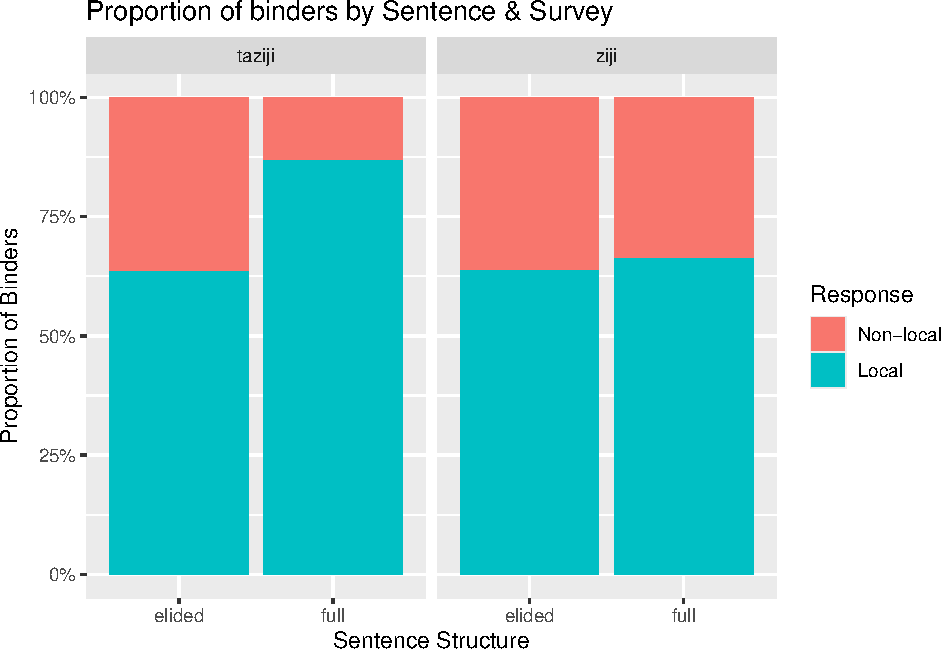
\includegraphics{index_files/figure-latex/unnamed-chunk-3-1.pdf}
First, the data is analyzed with a null model.

\begin{Shaded}
\begin{Highlighting}[]
\NormalTok{mod\_0 }\OtherTok{\textless{}{-}} \FunctionTok{glmer}\NormalTok{(}
  \AttributeTok{formula =}\NormalTok{ response }\SpecialCharTok{\textasciitilde{}} \DecValTok{1} \SpecialCharTok{+}\NormalTok{ (}\DecValTok{1} \SpecialCharTok{|}\NormalTok{ id),}
  \AttributeTok{family =} \FunctionTok{binomial}\NormalTok{(}\AttributeTok{link =} \StringTok{"logit"}\NormalTok{),}
  \AttributeTok{data =}\NormalTok{ dat1}
\NormalTok{  )}

\NormalTok{mod\_summary\_0 }\OtherTok{\textless{}{-}} \FunctionTok{tidy}\NormalTok{(mod\_0, }
                      \AttributeTok{effects =} \StringTok{"fixed"}\NormalTok{,}
                      \AttributeTok{conf.int =} \ConstantTok{TRUE}
\NormalTok{                      )}

\NormalTok{  knitr}\SpecialCharTok{::}\FunctionTok{kable}\NormalTok{(mod\_summary\_0, }\AttributeTok{digits =} \DecValTok{3}\NormalTok{ )}
\end{Highlighting}
\end{Shaded}

\begin{tabular}{l|l|r|r|r|r|r|r}
\hline
effect & term & estimate & std.error & statistic & p.value & conf.low & conf.high\\
\hline
fixed & (Intercept) & 0.902 & 0.07 & 12.839 & 0 & 0.764 & 1.039\\
\hline
\end{tabular}

As shown in the table above, there is a significant baseline preference for local binders (p \textless{} .001), consistent with theoretical predictions. However, this result does not provide information about the non-local binding.

Next, an inclusive model is used to analyze the data. A comparison with the null model shows that the inclusive model is a better fit, as indicated by its lower AIC value (3774.3).

\begin{Shaded}
\begin{Highlighting}[]
\NormalTok{mod\_1 }\OtherTok{\textless{}{-}} \FunctionTok{glmer}\NormalTok{(}
  \AttributeTok{formula =}\NormalTok{ response }\SpecialCharTok{\textasciitilde{}}\NormalTok{ sentence}\SpecialCharTok{*}\NormalTok{survey }\SpecialCharTok{+}\NormalTok{ (}\DecValTok{1} \SpecialCharTok{|}\NormalTok{ id),}
  \AttributeTok{family =} \FunctionTok{binomial}\NormalTok{(}\AttributeTok{link =} \StringTok{"logit"}\NormalTok{),}
  \AttributeTok{data =}\NormalTok{ dat1}
\NormalTok{  )}

\NormalTok{anova\_tidy\_1 }\OtherTok{\textless{}{-}} \FunctionTok{tidy}\NormalTok{(}\FunctionTok{anova}\NormalTok{(mod\_1, mod\_0, }
                         \AttributeTok{test=}\StringTok{"Chisq"}\NormalTok{)}
\NormalTok{                   )}
\NormalTok{knitr}\SpecialCharTok{::}\FunctionTok{kable}\NormalTok{(anova\_tidy\_1, }\AttributeTok{digits =} \DecValTok{3}\NormalTok{)}
\end{Highlighting}
\end{Shaded}

\begin{tabular}{l|r|r|r|r|r|r|r|r}
\hline
term & npar & AIC & BIC & logLik & minus2logL & statistic & df & p.value\\
\hline
mod\_0 & 2 & 3848.687 & 3860.828 & -1922.343 & 3844.687 & NA & NA & NA\\
\hline
mod\_1 & 5 & 3757.618 & 3787.972 & -1873.809 & 3747.618 & 97.069 & 3 & 0\\
\hline
\end{tabular}

The log-odds of a local-binder response is 0.5537 when both sentencefull and surveyziji are coded as 0, indicating that approximately 63\% of responses are local binders in the elided--taziji condition. The significant main effect of sentence (p \textless{} .001) suggests that local binders are more likely in full structures than in elided ones. The significant sentence × survey interaction shows that full structures substantially increase local-binder choice for \emph{taziji}, whereas \emph{ziji}'s binder preferences remain largely unchanged across structure types.

\begin{tabular}{l|l|r|r|r|r|r|r}
\hline
effect & term & estimate & std.error & statistic & p.value & conf.low & conf.high\\
\hline
fixed & (Intercept) & 0.554 & 0.073 & 7.540 & 0.000 & 0.410 & 0.698\\
\hline
fixed & sentencefull & 1.325 & 0.128 & 10.391 & 0.000 & 1.075 & 1.575\\
\hline
fixed & surveyziji & 0.005 & 0.104 & 0.052 & 0.959 & -0.198 & 0.209\\
\hline
fixed & sentencefull:surveyziji & -1.210 & 0.165 & -7.329 & 0.000 & -1.534 & -0.886\\
\hline
\end{tabular}

\begin{verbatim}
## [1] 0.6349936
\end{verbatim}

A restricted model is compared with the inclusive model. The AIC values show that the inclusive model yields a better fit. The interaction effect is significant.

\begin{Shaded}
\begin{Highlighting}[]
\NormalTok{mod\_2 }\OtherTok{\textless{}{-}} \FunctionTok{glmer}\NormalTok{(}
  \AttributeTok{formula =}\NormalTok{ response }\SpecialCharTok{\textasciitilde{}}\NormalTok{ sentence }\SpecialCharTok{+}\NormalTok{ survey }\SpecialCharTok{+}\NormalTok{ (}\DecValTok{1} \SpecialCharTok{|}\NormalTok{ id),}
  \AttributeTok{family =} \FunctionTok{binomial}\NormalTok{(}\AttributeTok{link =} \StringTok{"logit"}\NormalTok{),}
  \AttributeTok{data =}\NormalTok{ dat1}
\NormalTok{  )}
\NormalTok{anova\_tidy\_2 }\OtherTok{\textless{}{-}} \FunctionTok{tidy}\NormalTok{(}\FunctionTok{anova}\NormalTok{(mod\_2, mod\_1, }
                         \AttributeTok{test=}\StringTok{"Chisq"}\NormalTok{)}
\NormalTok{                   )}
\NormalTok{knitr}\SpecialCharTok{::}\FunctionTok{kable}\NormalTok{(anova\_tidy\_2, }\AttributeTok{digits =} \DecValTok{3}\NormalTok{)}
\end{Highlighting}
\end{Shaded}

\begin{tabular}{l|r|r|r|r|r|r|r|r}
\hline
term & npar & AIC & BIC & logLik & minus2logL & statistic & df & p.value\\
\hline
mod\_2 & 4 & 3800.260 & 3824.543 & -1896.130 & 3792.260 & NA & NA & NA\\
\hline
mod\_1 & 5 & 3757.618 & 3787.972 & -1873.809 & 3747.618 & 44.642 & 1 & 0\\
\hline
\end{tabular}

Significant main effects of sentence type (beta = 0.668, p \textless{} .001) and reflexive type (beta = --0.540, p \textless{} .001) on participants' binder choices are observed.

The log-odds of a local binder response is 0.839 when both sentencefull and surveyziji are 0. This corresponds to a predicted probability of approximately 70\% for a local binder response in elided sentences within the \emph{taziji} survey.

Holding surveyziji at 0, a one unit increase in sentencefull is associated with a 0.668 increase in log-odds. When holding sentencefull at 0, one unit increase in surveyziji is associated with a 0.540 decrease in log-odds. This means that the odds of a local binder response decrease by about 42\% in the \emph{ziji} survey compared to the \emph{taziji} survey.

\begin{tabular}{l|l|r|r|r|r|r|r}
\hline
effect & term & estimate & std.error & statistic & p.value & conf.low & conf.high\\
\hline
fixed & (Intercept) & 0.839 & 0.087 & 9.635 & 0 & 0.668 & 1.009\\
\hline
fixed & sentencefull & 0.668 & 0.103 & 6.486 & 0 & 0.466 & 0.870\\
\hline
fixed & surveyziji & -0.540 & 0.103 & -5.240 & 0 & -0.741 & -0.338\\
\hline
\end{tabular}

\section{4. Discussion}\label{discussion}

The inclusive model is selected for the analysis. Sentence type and reflexive type both show significant main effects on binder choice. While the result primarily reflects the choice of local binders, it also indirectly indicates a difference in non-local binder selection. Specifically, non-local binders are more likely to be chosen in the elided structure within the \emph{taziji} survey, supporting the prediction.

\newpage

\section{References}\label{references}

\phantomsection\label{refs}
\begin{CSLReferences}{1}{0}
\bibitem[\citeproctext]{ref-R-papaja}
Aust, F., \& Barth, M. (2024). \emph{{papaja}: {Prepare} reproducible {APA} journal articles with {R Markdown}}. \url{https://doi.org/10.32614/CRAN.package.papaja}

\bibitem[\citeproctext]{ref-R-tinylabels}
Barth, M. (2025). \emph{{tinylabels}: Lightweight variable labels}. \url{https://doi.org/10.32614/CRAN.package.tinylabels}

\bibitem[\citeproctext]{ref-R-base}
R Core Team. (2024). \emph{R: A language and environment for statistical computing}. Vienna, Austria: R Foundation for Statistical Computing. Retrieved from \url{https://www.R-project.org/}

\end{CSLReferences}


\end{document}
